\section{Finding High CNRE Clusters} \label{sect:finding}

Finding aggregate catchments --- pools of clients essentially directed toward
the same web resources --- necessarily involves finding sets of clients with high
CNRE measures between each other. Because CNRE is a measure of similarity, this
problem naturally lends itself to hierarchical clustering techniques \cite{murtagh1983survey}. 
We employ the complete linkage method to ensure cluster formation reflects commonalities
across all cluster members as opposed to potentially edge-specific properties.
Note that in all \emph{clustering} calculations, we opt to use the CNRE \emph{distance}
(\(1-\)CNRE) as defined in Section \ref{sect:cnre}.

Establishing hierarchical clusters requires that we have some definition of what
constitutes a \emph{high} or \emph{low} CNRE measure and at what threshold it is
appropriate to consider clients sufficiently similar such that they appear in
the same cluster. In this section, we explore the implications of various CNRE
values, as well as CNRE's relationship with other, well-established client grouping
systems: country, ASN, BGP prefix, and /24 prefix subnet.

\begin{figure*}
    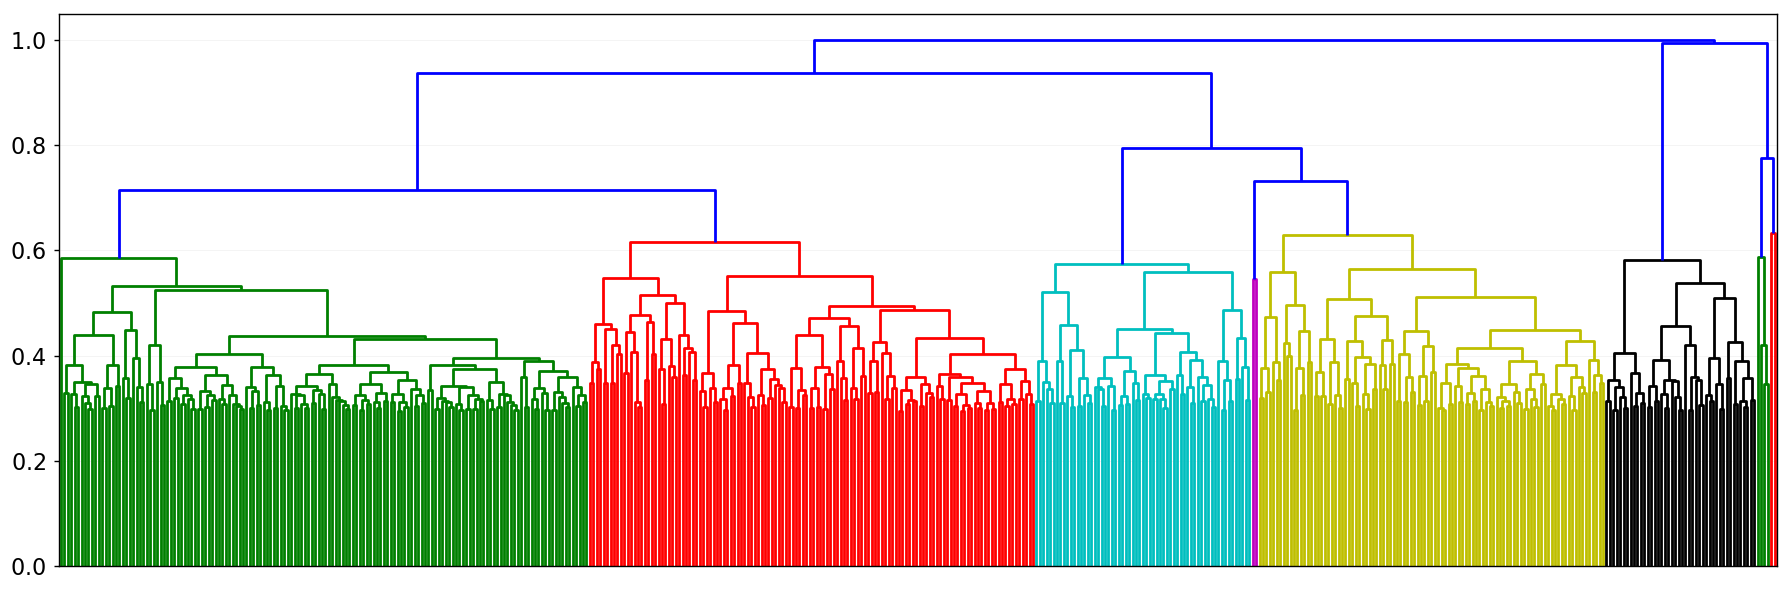
\epsfig{file=figs/dendrograms/v0.png, width=1\linewidth}
    \caption{Dendrogram of CNRE distance across all client pairs}
    \label{fig:dendrogram}
\end{figure*}

\subsection{Group Formation Patterns}
\label{s:formation}

Figure \ref{fig:dendrogram} presents a dendrogram derived from pairwise CNRE
distances across all clients and highlights three levels of distinct behavior
regarding the distribution of CNRE distances. First, in the uppermost portion of
the plot --- where CNRE distances are beyond a threshold of 0.63 --- we see
that distinctions between branches and their implied client groups become well
defined. Second, in the middle region of the tree, between CNRE distances of
0.25 and 0.63, we see that branches begin to fork unpredictably with shorter
changes in CNRE distance. Finally, in the lowest region of the plot, where CNRE
distances drop below 0.25, we see the amount of branching increase once again,
rapidly increasing the granularity of each branch as CNRE decreases further. 


\begin{figure*}
    \center
        \mbox{
            \begin{subfigure}[b]{0.33\linewidth}
                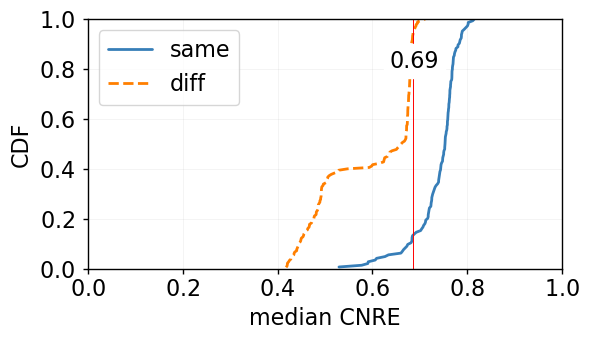
\epsfig{file=figs/cnre_vs_category/country.png, width=1\linewidth}
                \caption{country} 
                \label{fig:vscountry}
            \end{subfigure}
            \begin{subfigure}[b]{0.33\linewidth}
                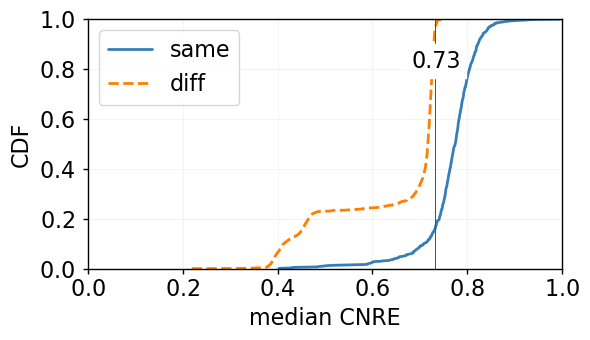
\epsfig{file=figs/cnre_vs_category/asn.png, width=1\linewidth}
                \caption{ASN} 
                \label{fig:vsasn}
            \end{subfigure}
            \begin{subfigure}[b]{0.33\linewidth}
                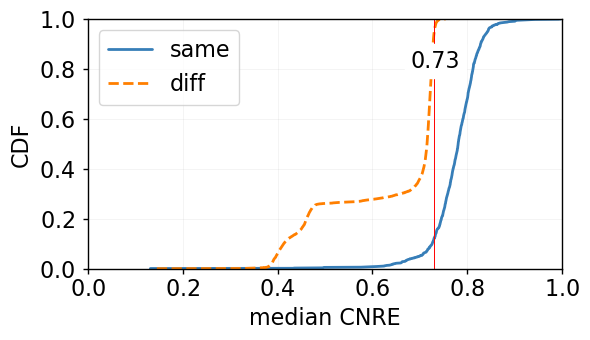
\epsfig{file=figs/cnre_vs_category/prefix.png, width=1\linewidth}
                \caption{BGP prefix} 
            \end{subfigure}
        }
    \caption{CDFs of CNREs across client sets with matching (same) and non-matching (diff) labels. 
    ``Same'' shows the CDF for the median CNRE distance across all client pairs matching a given label. 
    ``Diff'' shows the CDF for the median CNRE distance from each label group
    toward all other labels. The red, vertical line in each subfigure marks the
    95th percentile CNRE for for differing labels.}
    \label{fig:vslabel}

\end{figure*}

We compare established client group labeling schemes  ---
country, ASN, and BGP prefix --- to CNRE similarity between clients with
matching (\emph{e.g.}, same country) and differing (\emph{e.g.}, different
country) labels. Our findings are shown in Figure \ref{fig:vslabel}. The 95th percentile CNRE between groups with differing labels
is marked on each plot by a vertical red line; at this point,
differing and matching labels become distinguishable. For example, in Figure
\ref{fig:vasn}, a pair of clients with CNRE < 0.73 (see 0.27 in
Figure \ref{fig:dendrogram}, which uses CNRE distance) are likely from different
ASes, while clients with CNRE > 0.73 are likely from the AS. Note, however, that
\ref{fig:vslabel} uses \emph{median} values for all points shown. We analyze
this further in \ref{s:labelalgn}. 


Figures \ref{fig:vslabel} and \ref{fig:cnredist} together help provide a possible
explanation for three partiions observed in Figure \ref{fig:dendrogram}. In
Figure \ref{fig:vslabel}, we see that in all three subplots, the aforementioned
middle region of Figure \ref{fig:dendrogram} appears again, this time as a
plateau in both the ``Diff'' and ``Same'' curves. In this region, ``Diff'' and
``Same'' overlap significantly, rendering them indistinguishable. This transient
zone is given further context in Figure \ref{fig:cnredist}, where we shade each
country's median CNRE towards other countries (\emph{i.e.}, outbound
comparisons) --- the same data used to plot the
``Diff'' CDF in Figure \ref{fig:vscountry}. 

If a given country tends to have low CNREs between itself and all other
countries, this implies that the country is exposed to a more exclusive set of
web resources than its peers. For example, Australia, which, as shown in
\ref{fig:vscountry}, has a generally low CNRE with other countries, likely
utilizes very locale-targeted infrastructure given its relative distance from
more more broadly used network resources. Likewise, China, which is well
documented as having its Internet infrastructure deliberately disjoint from much
of the world (CITE great firewall, etc), also has a low CNRE with most other
countries. Conversely, we see most that countries within Europe and Africa tend
toward having higher CNREs with most other countries, implying that the majority
of web resources exposed in those regions are neither exclusive nor fine grained. 

\begin{figure}

    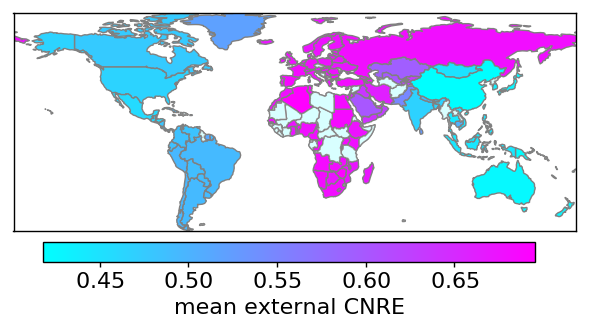
\epsfig{file=figs/cnre_country_uniqueness_map.png, width=1\linewidth}

    \caption{Choropleth with each country shaded by its median CNRE distance
    from all other countries.}
    \label{fig:cnredist}

\end{figure}

\subsection{Label Alignment}
\label{s:labelalgn}

Now that we have established some concept of what constitutes a ``high'' or
``low'' CNRE measure, we further consider CNRE in comparison to country, ASN,
and BGP prefix --- three labeling schemes commonly used group Internet clients.
Specifically, we wish to determine if the information captured by
CNRE (the extent to which clients are exposed to the same web resources) is
reasonably captured by any pre-existing system. If this were the case, one might
argue that the premise of treating CNRE as a separate system would be redundant
and arbitrarily complex. Therefore, we treat this subsection as a means of
validating and justifying the CNRE as a separate, currently unaddressed concept.

In Figure \ref{fig:ch}, we plot the completeness, homogeneity, and number of
clustesr for the aforementioned labeling schemes as we cluster clients in our
dataset, varying the CNRE distance threshold used for cluster formation. In
addition, we also mark, with a vertical line, the CNRE distance at which labels
become distinct (see Figure \ref{s:formation}), and we mark the number of labels
(\emph{i.e.}, the number countries, ASes, or BGP prefixes) present with a
horizontal line (using the righthand y-axis). 

If homogeneity and completeness, which together indicate how well cluster
membership aligns with a given labeling scheme, is not high, the CNRE-related
implications of a given label become ambiguous. We see in Figure \ref{fig:ch}
that for country and ASN, homogeneity and completeness are never simultaneously
high, rendering them unusable for determining CNRE on their own. BGP prefix,
however, requires more thorough consideration. In Figure \ref{fig:chbgp}

\begin{figure*}
    \center
        \mbox{
            \begin{subfigure}[b]{0.33\linewidth}
                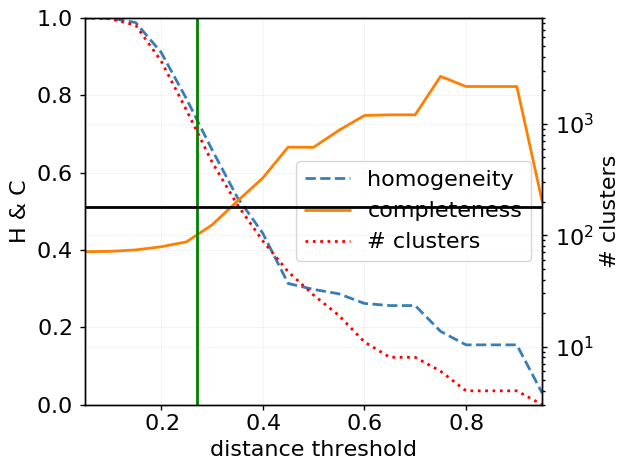
\epsfig{file=figs/completeness_vs_homogeneity/country.png, width=1\linewidth}
                \caption{country} 
            \end{subfigure}
            \begin{subfigure}[b]{0.33\linewidth}
                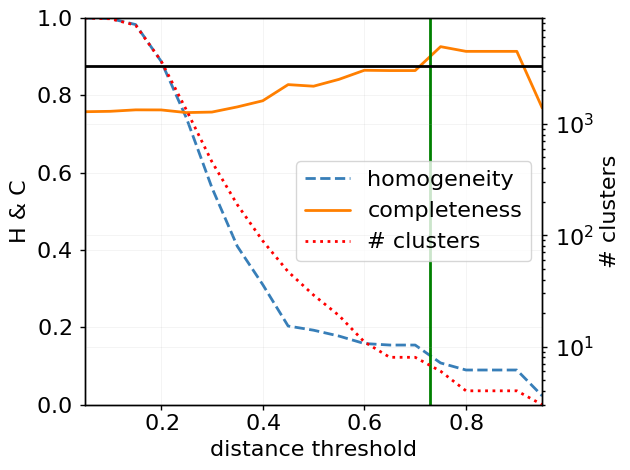
\epsfig{file=figs/completeness_vs_homogeneity/asn.png, width=1\linewidth}
                \caption{ASN} 
            \end{subfigure}
            \begin{subfigure}[b]{0.33\linewidth}
                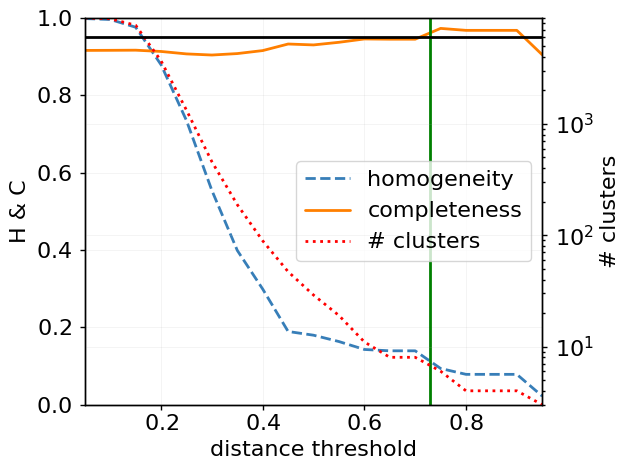
\epsfig{file=figs/completeness_vs_homogeneity/prefix.png, width=1\linewidth}
                \caption{BGP prefix} 
                \label{fig:chbgp}
            \end{subfigure}
        }
    \caption{Completeness, homogeneity, and number of clusters versus clustering
    distance threshold. The vertical line marks 0.27, the CNRE distance at which
    clients with differing labels become distinguishable, and the horizontal
    line denotes (using the right-side y-axis) the number of different real labels
    (for example, the number of countries) preesent in our data set for the
    given labeling scheme.}
    \label{fig:ch}
\end{figure*}


Figure \ref{fig:dendrogram} depicts the hierarchical clustering dendrogram based 
on pairwise CNRE distances.
This representation highlights the similarity of clients and different possible 
partitioning.
Each node in the tree is a cluster composed of the underneath denser clusters.
A horizontal cut in the dendrogram produces a partitioning of clients  for which
the dissimilarity of two probes in the same partition is not greater than the 
y-value where the cut is done. 

For example, the colored clusters in Figure~\ref{fig:dendrogram} are obtained 
with a cut at $y=0.65$.
This partitioning produces eight clusters including three small ones 
composed of outliers.
The five large clusters represent a very coarse partitioning of clients.
95\% of probes in the green cluster are from Europe and 4\% are from Africa 
(that is almost all African probes), the red cluster consists mainly of
German, Italian, and Russian probes (79\%), the blue cluster is mainly North and
South American probes (resp. 80\% and 18\%), the khaki cluster has mostly probes
from Asia and Oceania (resp. 67\% and 32\%), and the black cluster is mostly
North American probes (98\%).
As each cluster is composed of smaller and denser clusters, one can again partition
these clusters and form groups with clients having more network resources in common.
